% --------------------------------------------------------------------------------

\begin{exercise}

Sei $\Omega \subseteq \R^n$ ein beschränktes Gebiet mit $\partial\Omega \in C^1$.
Betrachten Sie die Poisson-Gleichung mit Neumann-Randbedingungen

\begin{align}
    \begin{cases}
    -\Delta u = f & \text{in } \Omega, \\
    \nabla u \cdot \nu = 0 & \text{auf}~ \partial\Omega,
    \end{cases}
    \label{neumann}
\end{align}

wobei $f \in L^2(\Omega)$.

\begin{enumerate}[label = \alph*)]

    \item Bestimmen Sie die schwache Formulierung für das Randwertproblem (1).

    \item Beweisen Sie die Existenz und Eindeutigkeit einer schwachen Lösung $u \in V$, wobei $V := \{v \in H^1(\Omega): \int_\Omega v(x)dx = 0\}$, für das RWP (1).
    \textit{Hinweis:}
    Poincaré-Ungleichung aus Aufgabe 4 von letzter Woche.

    \item Diskutieren Sie die Existenz und Eindeutigkeit von schwachen und klassischen Lösungen von (1), falls $\int_\Omega f(x)dx \neq 0$.

\end{enumerate}

\end{exercise}

% --------------------------------------------------------------------------------

\begin{solution}

\phantom{}

\includegraphicsboxed{PDEs/PDEs_-_Blatt_4_Aufgabe_4_poincaresche_Ungleichung.png}
\begin{enumerate}[label = \alph*)]

    \item Das RWP (1) entspricht genau (5.17) aus dem Skriptum mit

    \begin{align*}
        A := I, \quad b := 0, \quad c := 0, \quad g := 0.
    \end{align*}

    \includegraphicsboxed{PDEs/PDEs_-_(5-17).png}
    Wir führen die Umformulierung dennoch nochmal durch.
    Wir multiplizieren die Differentialgleichung mit $v \in H^1(\Omega)$, integrieren über $\Omega$ und integrieren partiell:

    \begin{align*}
        -\Delta u = f
        \implies
        (-\Delta u) v = f v
    \end{align*}

    \begin{align*}
        \implies
        \Int[\Omega]{f v}{x}
        =
        -\Int[\Omega]{(\Delta u) v}{x}
        =
        -\Int[\Omega]{(\Div \nabla u) v}{x}
        \stackrel
        {
            \mathrm{Gauß}
        }{=}
        \Int[\Omega]{\nabla u \cdot \nabla v}{x}
        -
        \Int[\partial \Omega]{\underbrace{(\nabla u \cdot \nu)}_0 v}{s}
    \end{align*}

    Dabei haben wir Satz 5.8 (Gauß für Sobolev-Funktionen) verwendet.

    \includegraphicsunboxed{PDEs/PDEs_-_Satz_5-8_Gauss_fuer_Sobolev-Funktionen.png}

    \begin{align*}
        a(u, v) := \Int[\Omega]{\nabla u \cdot \nabla v}{x},
        \quad
        F(v) := \Int[\Omega]{f v}{x}
    \end{align*}

    Also lautet die schwache Formulierung wie folgt:
    Finde $u \in H^1(\Omega)$, sodass

    \begin{align*}
        \Forall v \in H^1(\Omega):
        a(u, v) = F(v)
    \end{align*}

    \item $V$ ist, als $\Ker$ einer stetigen Funktion, ein Hilbertraum.

    \begin{align*}
        \abs{\Int[\Omega]{v}{x}}
        \leq
        \norm[L^1(\Omega)]{v}
        \stackrel
        {
            \mathrm{CSB}
        }{\leq}
        \norm[L^2(\Omega)]{1} \norm[L^2(\Omega)]{v}
        \leq
        \underbrace{|\Omega|^{1/2}}_{<\infty} \norm[H^1(\Omega)]{v}
    \end{align*}

    \begin{align*}
        V = \Ker \pbraces{H^1(\Omega) \to \R, v \mapsto \Int[\Omega]{v}{x}}
    \end{align*}

    Wir haben hier zwei Optionen.

    \begin{enumerate}[label = \arabic*.]

        \item Option (Satz 5.18 (Lemma von Lax-Milgram)):

        \begin{center}
            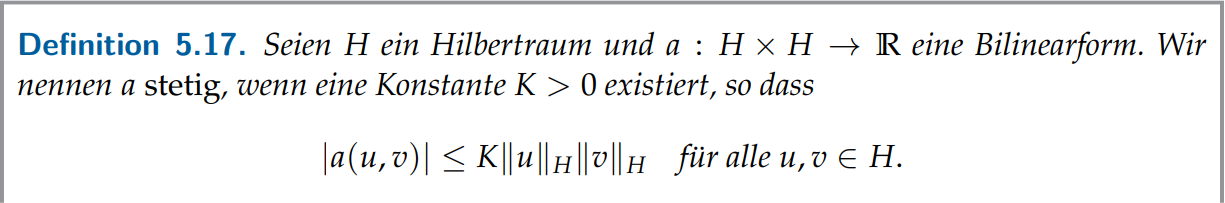
\includegraphics[width = 0.75 \textwidth]{PDEs/PDEs_-_Definition_5-17-1.png}
            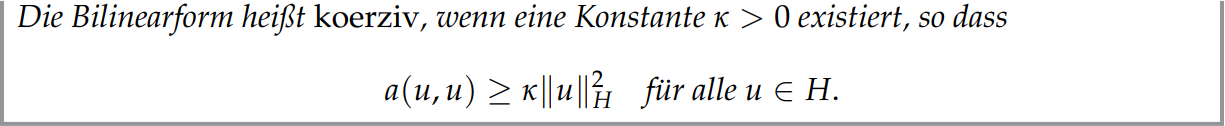
\includegraphics[width = 0.75 \textwidth]{PDEs/PDEs_-_Definition_5-17-2.png}
        \end{center}

        \includegraphicsunboxed{PDEs/PDEs_-_Satz_5-18_(Lemma_von_Lax-Milgram).png}

        \begin{itemize}

            \item Stetigkeit von $a$:

            \begin{align*}
                \abs{a(u, v)}
                \leq
                \norm[L^2(\Omega)]{\nabla u} \cdot \norm[L^2(\Omega)]{\nabla v}
                \leq
                \norm[H^1(\Omega)]{u} \norm[H^1(\Omega)]{v}
            \end{align*}

            \item Koerzivität von $a$:

            \begin{align*}
                a(u, u)
                =
                \Int[\Omega]{\nabla u \nabla u}{x}
                =
                \norm[L^2(\Omega)]{\nabla u}^2
                \stackrel
                {
                    \mathrm{P}
                }{\geq}
                \frac{1}{C^2 + 1}
                \pbraces
                {
                   \norm[L^2(\Omega)]{u} + \norm[L^2(\Omega)]{\nabla u}^2
                }
                =
                \frac{1}{C^2 + 1} \norm[H^1(\Omega)]{u}
            \end{align*}

            \item Stetigkeit von $F$:

            \begin{align*}
                \abs{F(v)}
                =
                \abs{\Int[\Omega]{f v}{x}}
                \leq
                \Int[\Omega]{\abs{f v}}{x}
                =
                \norm[L^1(\Omega)]{f v}
                \stackrel
                {
                \mathrm{CSB}
                }{\leq}
                \norm[L^2(\Omega)]{f} \norm[L^2(\Omega)]{v}
                \leq
                \norm[L^2(\Omega)]{f} \norm[H^1(\Omega)]{v}
            \end{align*}

        \end{itemize}

        \item Option (Satz 5.1 (Darstellungssatz von Riesz)):

        \includegraphicsunboxed{PDEs/PDEs_-_Satz_5-1_(Darstellungssatz_von_Riesz).png}


        Aus der 2. poincaréschen Ungleichung erhalten wir $\Exists C > 0: \Forall v \in V:$

        \begin{align*}
            \norm[L^2(\Omega)]{\nabla v}^2
            \leq
            \norm[H^1(\Omega)]{\nabla v}^2
            =
            \norm[L^2(\Omega)]{v - \overline{v}}^2 + \norm[L^2(\Omega)]{\nabla v}^2
            \stackrel
            {
                \mathrm{P}
            }{\leq}
            (C^2 + 1) \norm[L^2(\Omega)]{\nabla v}^2.
        \end{align*}

        Daher definiert $a: V \times V \to \R$ ein zu $(\cdot, \cdot)_{H^1(\Omega)}$ äquivalentes Skalarprodukt auf $V$.
        Das macht $(V, a)$ zu einem Hilbertraum.

        \begin{align*}
            \implies
            a \sim (\cdot, \cdot)_{H^1(\Omega)} ~\text{auf}~ V
            \implies
            (V, a) ~\text{Hilbertraum}
        \end{align*}

        Nicht zuletzt ist $F \in V^\prime$ ein lineares und (bzgl. $a$) stetiges Funktional.

        \begin{multline*}
            \abs{F(v)}
            =
            \abs{\Int[\Omega]{f v}{x}}
            \leq
            \Int[\Omega]{\abs{f v}}{x}
            \stackrel
            {
                \mathrm{CSB}
            }{\leq}
            \norm[L^2(\Omega)]{f} \norm[L^2(\Omega)]{v} \\
            =
            \norm[L^2(\Omega)]{f} \norm[L^2(\Omega)]{v - \overline{v}}
            \stackrel
            {
                \mathrm{P}
            }{\leq}
            \norm[L^2(\Omega)]{f} C \norm[L^2(\Omega)]{\nabla v}
        \end{multline*}

    \end{enumerate}

    Laut dem Lemma von Lax-Milgram, bzw. Darstellungssatz von Riesz existiert nun genau ein $u \in V$, sodass $a(u, v) = F(v)$ für alle $v \in V$.

    \begin{align*}
        \implies
        \ExistsOnlyOne u \in V:
        \Forall v \in V:
        a(u, v) = F(v)
    \end{align*}

    Damit $u$ auch eine schwache Lösung in $H^1(\Omega)$ (und nicht nur in $V$) ist, müssen wir diese Gleichheit jetzt noch für alle $w \in H^1(\Omega)$ zeigen.
    Sei also $w \in H^1(\Omega)$, dann ist $w - \overline{w} \in V$.

    \begin{align*}
        w \in H^1(\Omega)
        \implies
        \Int[\Omega]{w - \overline{w}}{x}
        =
        \Int[\Omega]{w}{x} - \Int[\Omega]{\overline{w}}{x}
        =
        \Int[\Omega]{w}{x} - |\Omega| \overline{w}
        =
        0
        \implies
        w - \overline{w} \in V
    \end{align*}

    Damit können wir den oberen Teil auf $w - \overline{w}$ anwenden.

    \begin{multline*}
        a(u, w)
        =
        a(u, w) - \Int[\Omega]{\nabla u \underbrace{\nabla \overline{w}}_0}{x}
        =
        a(u, w) - a(u, \overline{w})
        =
        a(u, w - \overline{w}) \\
        =
        F(w - \overline{w})
        =
        F(w) - F(\overline{w})
        =
        F(w) - \Int[\Omega]{f \overline{w}}{x}
        =
        F(w) - \overline{w} \underbrace{\Int[\Omega]{f}{x}}_0
        =
        F(w)
    \end{multline*}

    \item Für $\Int[\Omega]{f(x)}{x} \neq 0$ und eine schwache Lösung $u \in H^1(\Omega)$ folgt
    nach Integrieren der Differentialgleichung mit Satz 5.8 (Gauß für Sobolev-Funktionen) ein Widerspruch!

    \begin{align*}
        0
        \neq
        \Int[\Omega]{f(x)}{x}
        =
        -\Int[\Omega]{\Delta u}{x}
        =
        \Int[\partial \Omega]{\underbrace{\nabla u \cdot \nu}_0}{s}
        =
        0
    \end{align*}

    Also kann es in dem Fall keine schwachen und insbesondere keine klassischen Lösungen geben.

\end{enumerate}

\end{solution}

% --------------------------------------------------------------------------------
